\chapter{Object Detection using Computer Vision}

\paragraph*{}
Based on the progress documented in the first report, there were previously identified issues with the object detection system, specifically related to the HSV (Hue, Saturation, Value) color code, which affected the robot's ability to reliably detect the yellow box as intended. In this phase of the project, those issues have been resolved, leading to improved performance and accuracy in object detection.

\paragraph*{}
The setup remains consistent with the original object detection simulation, utilizing an RGB camera and a display. While a rangefinder is installed alongside these devices, it is not actively used for object detection. Instead, its placement at the same location as the other two devices serves to simulate an RGB-D camera, which combines both color and depth data. This setup also allows for flexibility in case we need to experiment with using the rangefinder for depth-based testing in future iterations.

\paragraph*{}
One of the key improvements made was adjusting the luminosity settings within the WeBots simulation. By increasing the plan's luminosity from 1 to 1.2, the colors in the environment became brighter and more closely resembled real-world conditions. This adjustment was critical because it made the HSV color code range of yellow in the simulation more realistic, aligning it more accurately with the yellow detected in real-world scenarios. This fine-tuning allowed the robots to detect yellow objects as intended, bridging the gap between simulated and real-world color perception.

\paragraph*{}
To illustrate this, the color code for yellow in HSV space was adjusted and now ranges between (70, 100, 0) and (90, 255, 255). This range was carefully selected based on real-world observations, ensuring that the simulation's lighting conditions produce a color that matches this HSV range after increasing luminosity.

\paragraph*{}
For the computer vision component, the approach employed involves creating a mask over the detected object. Once the mask is generated, a bounding box is drawn around the masked area to identify the detected object clearly. This bounding box serves as a visual marker, allowing the robots to focus on the target.


\paragraph*{}
After the bounding box is created, the robots in the simulation are programmed to locate the detected object by centering it within the frame of the camera. Each robot maneuvers in a circular motion, adjusting its position until the bounding box appears in the center of the camera's frame. To achieve this, the distance between the left side of the frame and the leftmost point (x) of the bounding box must be equal to the distance between the right side of the frame and the right edge of the bounding box (x+w). Once these distances are balanced, the robot will halt its motion. This ensures that all robots are facing directly towards the detected object, optimizing their orientation for subsequent actions.

\paragraph*{}
Overall, these enhancements have significantly improved the object detection system. The robots can now reliably detect and align themselves with yellow objects, ensuring smoother and more accurate performance in the simulated environment. The adjustments made to the HSV color range and the environmental luminosity were critical steps that contributed to this progress.

\begin{figure}[H]
    \centering
    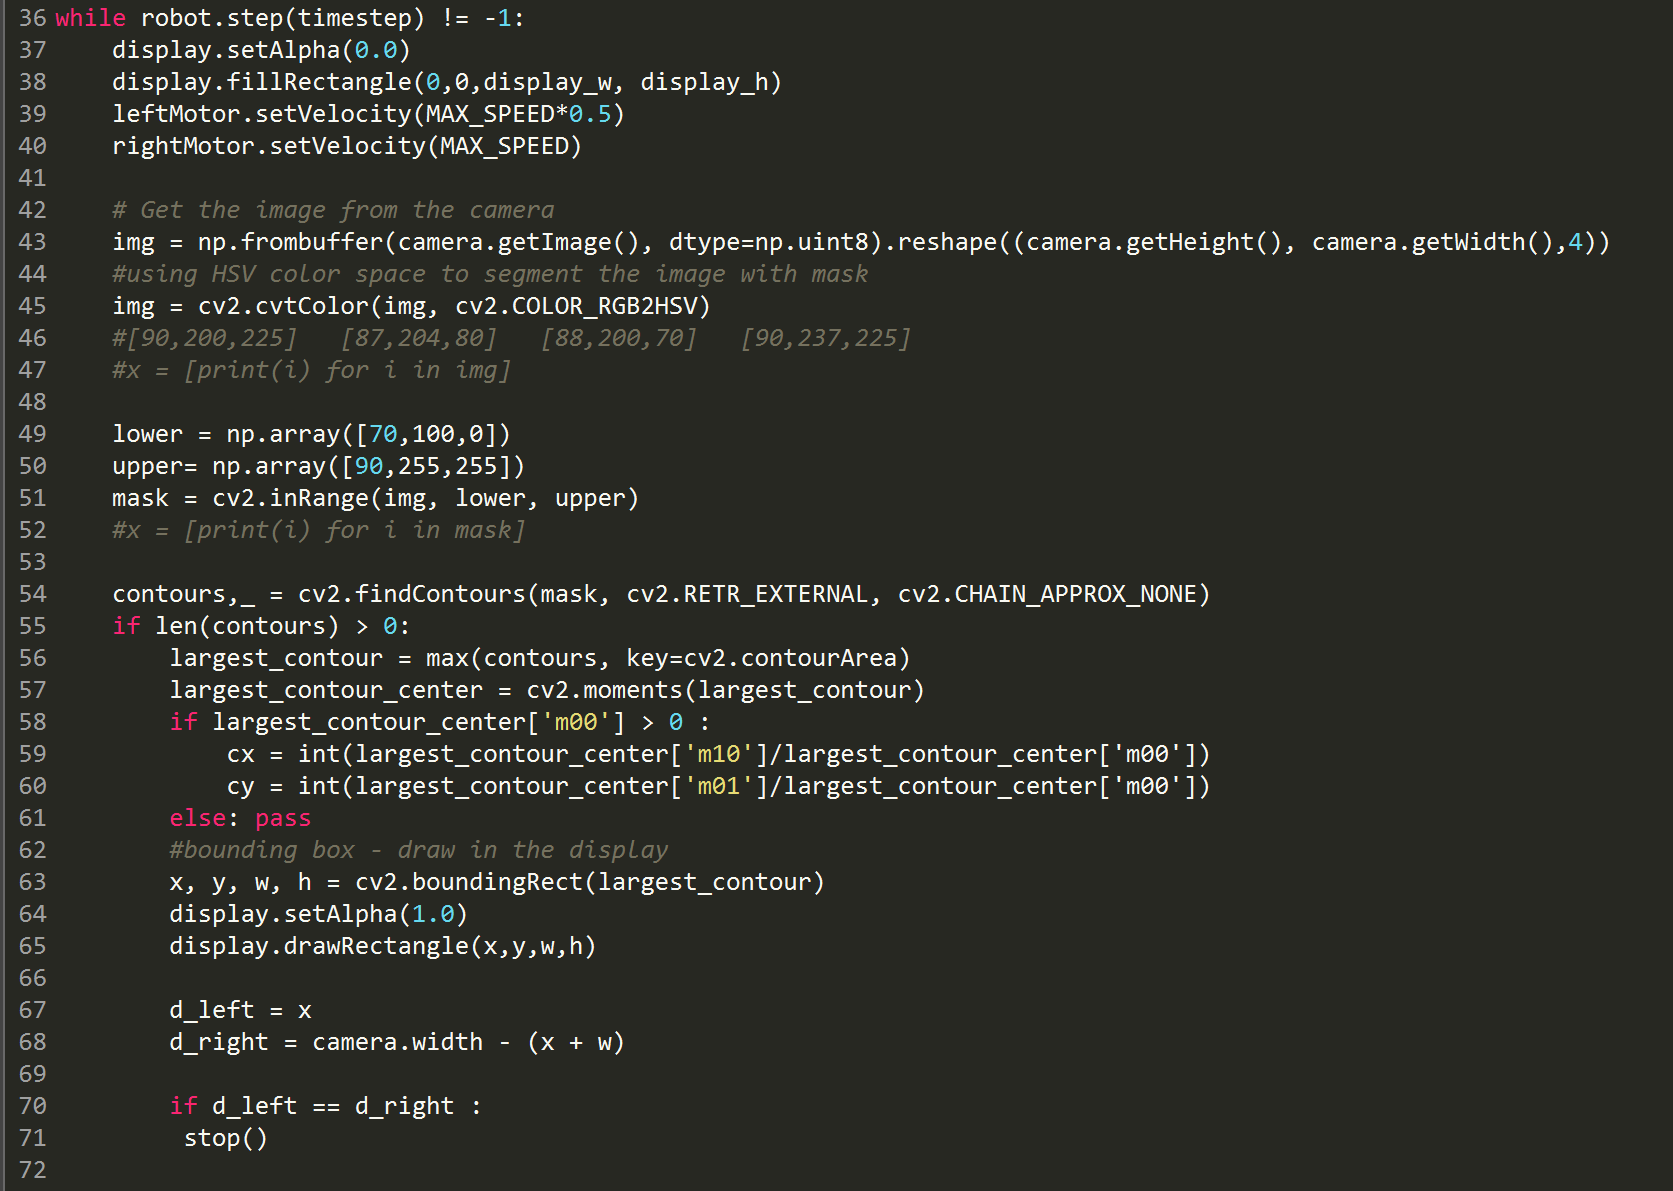
\includegraphics[width=0.6\linewidth]{assets/images/object_detection/figure1.png}
    \caption{Main loop of the robot controller for performing object detection}
    \label{fig:object detection figure 1.} 
\end{figure}

\paragraph*{}
For the computer vision part, the approach utilized in this area is to create a mask over the detected object followed by drawing a bounded box around the detected object or the mask that is created.

\paragraph*{}
After the bounded box is created, our robots in the simulation aim to locate the detected object in the middle of the frame (camera). So all robots will basically move , in this case in circular motion, until the bounded box is located in the middle of the frame. We only consider the distance between the left side of the frame to the leftmost point (x) of the bounded box which has to be equal to the distance between the right side of the frame and the right side if the bounded box(x+w). Once the distance between two parts are equal, the robot will stop the motion. Thus all robots will face towards the detected object as shown in Figure 2.

\begin{figure}[H]
    \centering
    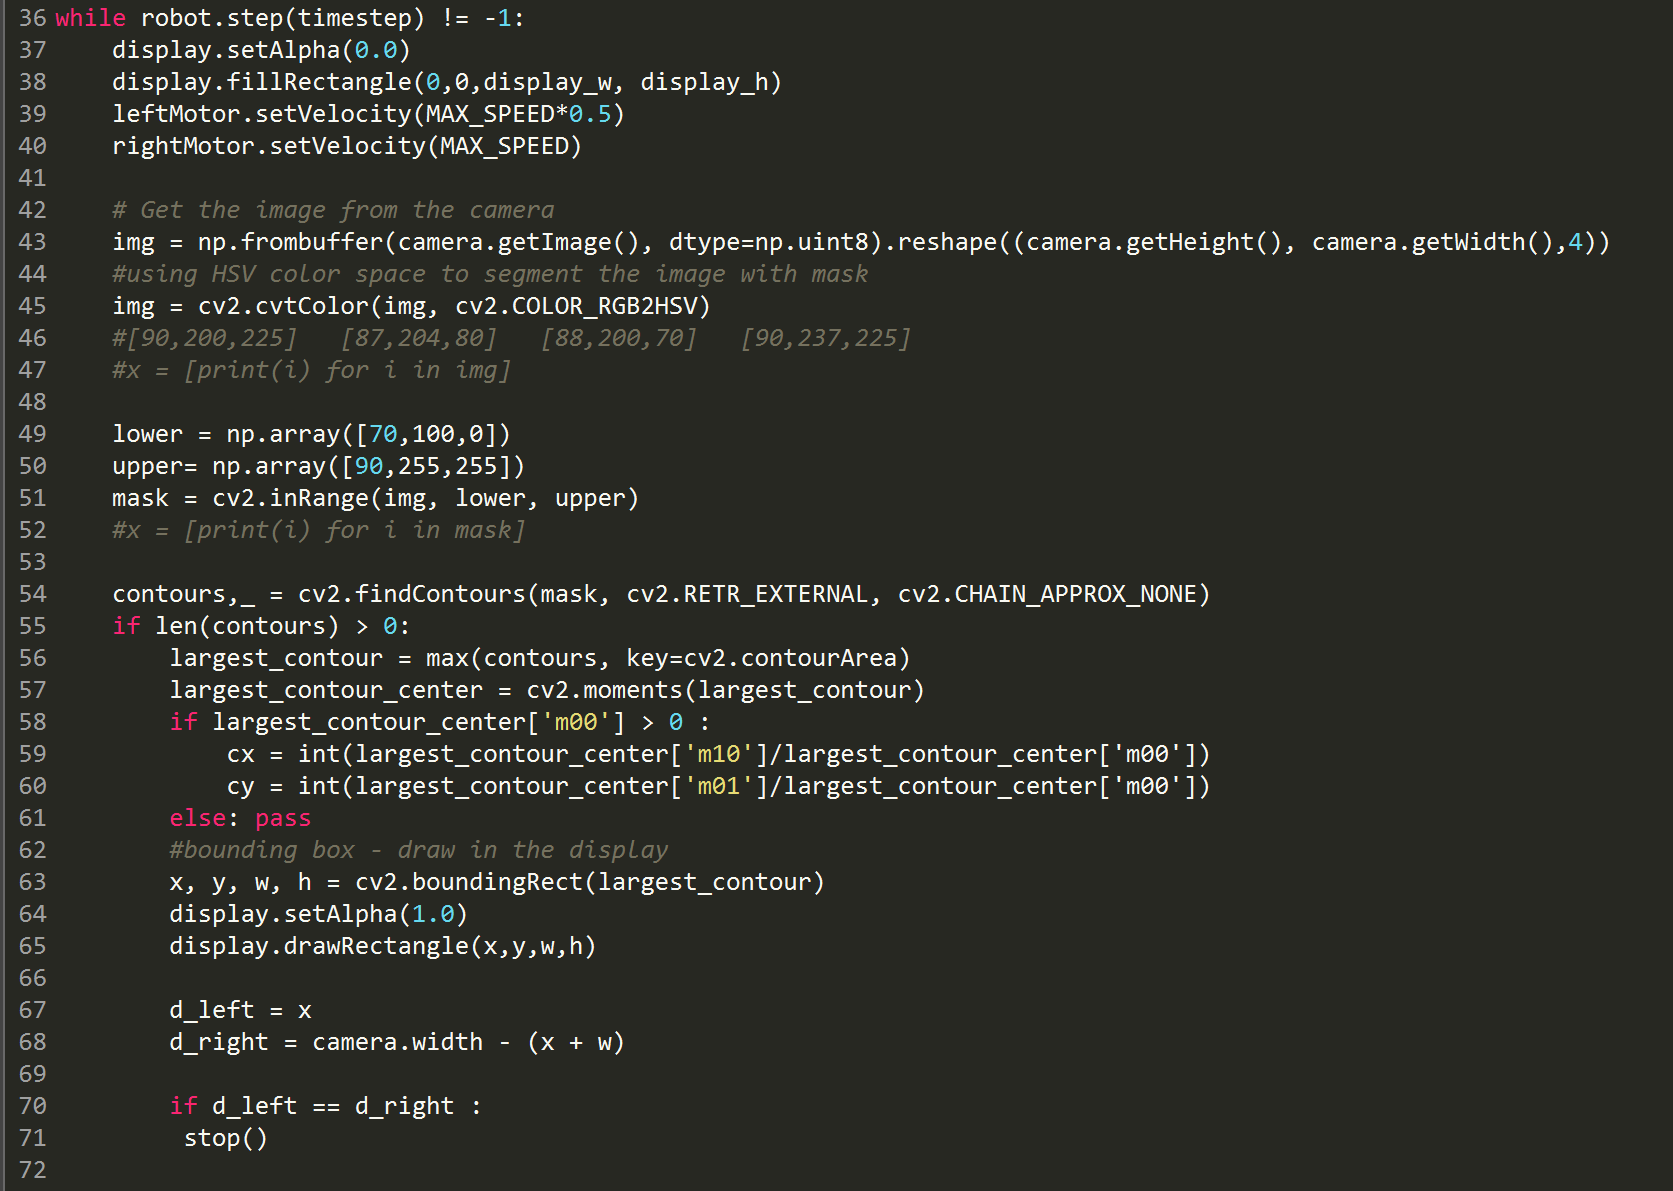
\includegraphics[width=0.6\linewidth]{assets/images/object_detection/figure1.png}
    \caption{The final position of each robot after the yellow box is detected and located in the middle of the frame}
    \label{fig:object detection figure 2.} 
\end{figure}
